\chapter{KAJIAN PUSTAKA}

\section{\textit{Clustering} Siswa}

\textit{Clustering} atau pengelompokan merupakan salah satu jenis informasi yang diperoleh dari data mining selain \textit{associations, sequences, classification} dan \textit{forecasting}. Salah satu bidang terpenting yang berfokus pada pemahaman sifat-sifat kumpulan data dan juga pada proses analitis penemuan pengetahuan dalam basis data (KDD), atau pemahaman pengetahuan dalam basis data, adalah penambangan data.  Data mining diterapkan pada kumpulan data yang sangat besar menggunakan algoritma terawasi dan tidak terawasi.  Data mining memungkinkan analisis data atau informasi dalam jumlah besar untuk mengidentifikasi pola dan menggunakan pola tersebut dalam memprediksi periode studi di masa depan.  Salah satu teknik data mining untuk mengklasifikasikan sekelompok item ke dalam kelompok sasaran adalah klasifikasi \citep{Oluwaseun2019}.

Menurut \citep{Adodo2011}, \textit{Clustering} siswa berdasarkan kesamaan kemampuan memiliki beberapa nilai positif diantaranya: meningkatkan kemampuan akademis siswa, membantu guru lebih mudah dalam mengajar, mempermudah guru dalam memberikan motivasi kepada siswa berprestasi dan kurang berprestasi dalam akademisnya, siswa berprestasi akademik rendah akan merasa lebih nyaman dengan teman-teman yang memiliki kemampuan sama, membantu guru dalam pemberian metode pengajaran yang sesuai dengan kemampuan kelompok siswa serta dapat mengoptimalkan waktu. Selain itu menurut, adanya \textit{Clustering} kemampuan dari segi akademis terhadap siswa memiliki manfaat yaitu kebutuhan Pendidikan siswa terpenuhi, meningkatnya hasil yang diraih siswa, tercapainya keinginan orangtua yang mana anaknya ingin digabungkan dengan siswa dengan kemampuan akademis yang sama, dan \textit{Clustering} ini dapat memaksimalkan sarana pembelajaran. Namun, terdapat kekurangan terhadap \textit{Clustering} siswa berdasarkan kemampuan yakni: harapan guru terhadap kesamaan prestasi siswa menurun, akan selalu ada stigma negatif terhadap kelas rendah, susahnya mengatur jam pelajaran di sekolah, dan tidak jarang permasalahan prilaku timbul di kelompok siswa kelas rendah serta dikarenakan Teknik \textit{Clustering} siswa masih dilakukan dengan cara manual, sebagian orangtua merasa takut dan cemas jika terdapat kekeliruan dalam \textit{Clustering} anak mereka oleh guru.

Teknik \textit{Clustering} data dengan cara mengelompokan data yang mirip satu sama lain dan berbeda dengan kelompok lain \citep{Han2011}. \textit{Clustering} mengumpulkan data yang tidak berlabel membentuk kelompok dengan karakter data yang mirip. Dalam kajian kepustakaan yang dilakukan, peneliti menemukan tiga metode yang dapat melakukan \textit{Clustering} yaitu \textit{Clustering Fuzzy C-Means} (FCM), \textit{K-Means}, dan SOM.

K-Means merupakan algoritma yang dapat mengolah data dalam jumlah yang besar dengan efektif. Namun, terdapat kelemahan dalam K-Means yaitu menentukan titik awal centroid  \citep{Nugroho2012}. Untuk menangani permasalahan tersebut, banyak peneliti yang menggabungkan metode K-Means dengan \textit{Self Organizing Map} (SOM). Dalam penelitian tentang gabungan dari metode SOM dan K-Means, SOM berfungsi untuk menentukan titik awal centroid, kemudian K-Means berfungsi untuk menentukan hasil akhir \textit{Clustering}.

Kemudian teknik \textit{Clustering} selanjutnya adalah SOM. SOM digunakan untuk mengelompokan data berdasarkan karakteristik/fitur-fitur data \citep{Lestari2014}. SOM menggunakan metode pembelajaran unsupervised yang proses pelatihannya tidak memerlukan pengawasan. Dalam SOM klasik terdapat perbaruan bobot yang dilakukan setelah data masuk.

Terdapat pengembangan SOM klasik yang bersifat statis yaitu \textit{Batch Learning Self Organizing Map} (BLSOM). Dalam BLSOM perbaruan bobot dilakukan di akhir dalam satu epoch sehingga proses pembelajaran SOM menjadi lebih cepat \citep{VasighiAmini2017}. SOM dan BLSOM merupakan varian som yang bersifat statis, yang berarti jumlah neuron output di inisialisasi pada awal pelatihan dan jumlah neuron output akan sama pada akhir pelatihan.

Penentuan jumlah neuron yang lebih tepat dalam AMSOM tidak penting, karena jumlah neuron akan disesuaikan selama proses pelatihan \citep{vandenHerik2017}. Selanjutnya GSOM, GSOM memberikan struktur yang fleksibel dalam pembentukan map, pada awal pelatihan map berukuran kecil dan di akhir pelatihan ukuran map membesar sesuai dengan penambahan neuron \citep{VasighiAmini2017}.

Penambangan atau eksplorasi data adalah bagian dari area penelitian terbaru yang lebih luas dalam Kecerdasan Buatan dan Pemrosesan dan Manajemen Informasi atau dikenal sebagai \textit{Knowledge Discovery in Database} (KDD). Tujuannya untuk mengidentifikasi informasi atau pengetahuan baru dari database di mana dimensi atau jumlah data sangat besar sehingga melampaui pemahaman manusia. MST digunakan untuk menganalisis basis data transformator daya dari satu dari penyedia energi listrik di Jepang. Evaluasi kelompok dihasilkan oleh SOM biasanya dilakukan oleh mata manusia. Karena sifatnya kualitatif alam, evaluator dapat melebih-lebihkan atau meremehkan jumlah kelompok yang terbentuk di peta. Dengan pendekatan ini, tepat jumlah kelompok yang dihasilkan oleh peta tidak dapat dikonfirmasi karena salah tafsir dari ekspresi tingkat abu-abu \citep{Tokutaka2001}.

Penelitian tentang teknik visualisasi menggunakan SOM dan MST. Metode ini dapat mengungkapkan kelompok barang serupa, berdasarkan graf yang dibangun baik dari data input, atau node SOM. Evaluasi visualisasi, dan membandingkannya dengan metode graf kerapatan, dan menemukannya untuk mengungkapkan informasi serupa. Visualisasi tidak bergantung pada parameter pengguna tertentu, yang bermanfaat bagi pengguna pemula. Metode operasi pada simpul SOM umumnya memiliki waktu komputasi yang lebih rendah daripada metode graf kepadatan, karena jumlah node dalam SOM umumnya besarnya lebih kecil dari jumlah sampel data \citep{MayerRauber2010}.

Penelitian terdahulu tentang SOM-MST dan bukan dalam bidang pendidikan serta dataset yang digunakan bukan merupakan log data, sehingga penulis mengusulkan penelitian \textit{ SOM-m-ary-Tree} dalam bidang pendidikan menggunakan log data aktivitas siswa dalam media pembelajaran Monsakun.

\section{Jaringan Saraf Tiruan}

Jaringan saraf tiruan adalah sistem pemrosesan informasi yang memiliki karakteristik kinerja tertentu yang sama dengan jaringan saraf biologis. Jaringan saraf tiruan telah dikembangkan sebagai generalisasi model matematika dari kognisi manusia atau biologi saraf, berdasarkan pada asumsi bahwa:

\begin{enumerate}
	\item Pemrosesan informasi terjadi pada banyak elemen sederhana yang disebut
	\textit{neuron}.
	\item Sinyal dilewatkan di antara neuron melalui tautan koneksi.
	\item Setiap tautan koneksi memiliki bobot terkait, yang, dalam jaringan saraf tipikal, mengalikan sinyal yang ditransmisikan.
	\item Setiap \textit{neuron} menerapkan fungsi aktivasi ke \textit{input} netto (jumlah sinyal input
	tertimbang) untuk menentukan sinyal \textit{output}-nya.
\end{enumerate}

Jaringan saraf ditandai (1) pola koneksi antara \textit{neuron} (disebut arsitekturnya), (2) metode penentuan bobot pada koneksi (disebut pelatihan, atau pembelajaran, algoritme), dan (3) fungsi aktivasi.

Karena apa yang membedakan jaringan saraf (buatan) dari pendekatan lain dalam pemrosesan informasi memberikan pengantar tentang bagaimana dan kapan menggunakan jaringan saraf.

Jaringan saraf terdiri dari sejumlah besar elemen pemrosesan sederhana yang disebut \textit{neuron}, unit, sel, atau node. Setiap \textit{neuron} terhubung ke \textit{neuron} lain melalui tautan komunikasi terarah, masing-masing dengan bobot terkait. Bobot mewakili informasi yang digunakan oleh internet untuk menyelesaikan masalah.

\begin{figure}[h]
	\centering
	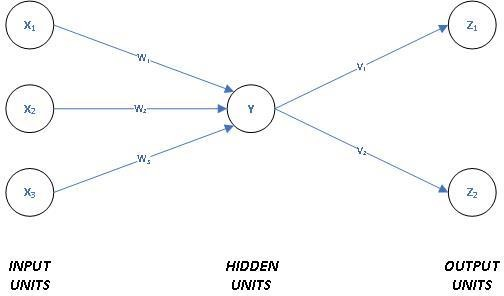
\includegraphics[width=0.5\textwidth]{Gambar/strukturdata}
	\caption{Struktur Dasar Jaringan Saraf Tiruan}
	\label{fig:g2}
\end{figure}

Pada \ref{fig:g2} dijelaskan bahwa setiap \textit{neuron} memiliki keadaan internal, yang disebut tingkat aktivasi atau aktivitas, yang merupakan fungsi dari input yang telah diterima. Biasanya, \textit{neuron} mengirimkan aktivasinya sebagai sinyal ke beberapa \textit{neuron} lain. Penting untuk dicatat bahwa \textit{neuron} hanya dapat mengirim satu sinyal pada satu waktu, meskipun sinyal itu disiarkan ke beberapa \textit{neuron} lain.

\section{Kohonen \textit{Self-Organizing Maps} (SOM)}

\textit{Self-Organizing Map} (SOM) pertama kali diperkenalkan oleh Teuvo Kohonen pada tahun 1982. SOM merupakan salah satu model dari Jaringan Saraf Tiruan. SOM merupakan salah satu tool untuk menangani data yang sangat besar, 
dimana data yang \textit{high-dimensional} data dapat divisualisasikan menjadi \textit{low-dimensional} data, atau mengurangi dimensi \textit{vector} \citep{Kohonen2013}.

Metode pembelajaran yang digunakan SOM adalah tanpa bimbingan dari suatu data \textit{input}-target atau \textit{unsupervised learning}. Artinya, sebuah jaringan akan belajar dengan dibekali pengetahuan dasar (parameter-parameter jaringan) tanpa adanya pengetahuan awal lebih dulu mengenai segmen dan karakteristiknya serta tanpa harus mengetahui berapa kelompok yang akan dibentuk, dan kemudian mengorganisasikan sendiri hubungan-hubungan interkoneksi dalam dirinya atas masukan yang diberikan sehingga dengan demikian target tidak dibutuhkan.

Di dalam SOM terdapat koneksi antara input-input dengan node-node yang memiliki bobot masing-masing. Sehingga, bobot yang telah ditentukan berkorespondensi untuk setiap node yang ada \citep{StefanovicKurasova2014a}. Himpunan bobot membentuk suatu vektor yang biasanya disebut neuron, dimana terdapat sejumlah baris dan kolom (dalam kasus ini, topologi yang diguanakn adalah topologi persegi panjang). Tujuan utama dari metode SOM ini adalah untuk mempertahankan topologi data multidimensi ketika mereka ditransformasikan menjadi ruang dimensi yang lebih rendah. Biasanya, metode SOM sendiri digunakan untuk mengelompokkan, mengklasifikasikan, dan memvisualisasikan berbagai jenis \textit{dataset}. SOM hanya dapat menangani data numerik, jadi pertama-tama, kita harus mengubah segala jenis dataset menjadi dataset     berekspresi     numerik.     Misalkan,     kita     memiliki    \textit{dataset} $X = \{ X_1, X_2, \ldots, X_n \}$, dimana     setiap     item     data     memiliki     beberapa     fitur $x_1, x_2, x_3, \ldots, x_n \ $ i.e. $\ X_i = \{ X_{i1}, X_{i2}, \ldots, X_{in} \}$.
Sehingga $X_i$ adalah vector dari $n$ ruang dimensi (\textit{n-dimensional data}), $X_i \in \mathbb{R}^n$. Semua \textit{dataset} dijadikan SOM sebagai matrix:

\[
\begin{bmatrix}
	X_{11} & X_{12} & \cdots & X_{1n} \\
	X_{21} & X_{22} & \cdots & X_{2n} \\
	\vdots & \vdots & \ddots & \vdots \\
	X_{N1} & X_{N2} & \cdots & X_{Nn}
\end{bmatrix}
\]

Berikut $X_{pl}$ merupakan nilai komponen dari vektor $X_i$, dimana $i = 1, 2, \ldots, N$, $l = 1, 2, \ldots, n$. 
Nilai $N$ merupakan jumlah vektor input yang dianalisis dan nilai $n$ merupakan jumlah komponen. 
Proses pembelajaran algoritme SOM dimulai dari inisialisasi komponen vektor (\textit{neuron}). 
Mereka dapat diinisialisasi secara acak (biasanya nilai-nilai ini adalah angka acak dari interval $(0, 1)$) 
atau oleh komponen utama $W_{ij}$. 
Pada setiap langkah pembelajaran, vektor masukan $X_i \in \{ X_1, X_2, \ldots, X_N \}$ dilewatkan ke SOM. 
Vektor $X_i$ dibandingkan dengan semua \textit{neuron} $W_{ij}$. 
Biasanya perhitungan bobot jarak menggunakan metode \textit{Euclidean Distance} antara vektor input $X_i$ 
dibandingkan dengan masing-masing neuron $W_{ij}$. 
Vektor (\textit{neuron}) $W_w$ dengan jarak \textit{Euclidean} minimal ke $X_i$ ditetapkan sebagai neuron pemenang 
(\textit{best match unit}) \citep{StefanovicKurasova2014a}. 
Semua komponen neuron diadaptasi sesuai dengan aturan pembelajaran berikut:

\[
W_{ij}(\text{new}) = W_{ij}(\text{old}) + h_w \big( X_i - W_{ij}(\text{old}) \big)
\]

\section{Arsitektur SOM}

Arsitektur SOM merupakan jaringan yang terdiri dari dua lapisan, yaitu lapisan \textit{input} dan \textit{output}.

\begin{figure}[h]
	\centering
	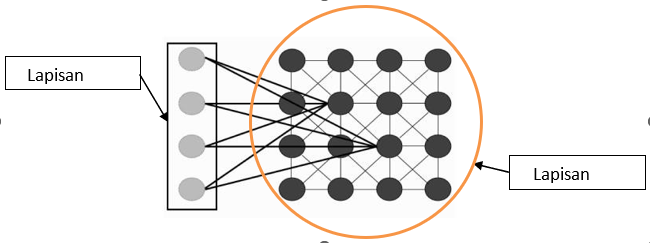
\includegraphics[width=0.8\textwidth]{Gambar/arsitektursom}
	\caption{Arsitektur SOM}
	\label{fig:g3}
\end{figure}

Pada \ref{fig:g3} dijelaskan bahwa setiap \textit{neuron} dalam lapisan \textit{input} terhubung dengan setiap \textit{neuron} pada lapisan \textit{output}. Setiap \textit{neuron} pada lapisan \textit{output} merepresentasikan kelompok dari \textit{input} yang diberikan.

\section{Parameter Pembelajaran (\textit{Learning Parameters})}

Hasil dari SOM bergantung pada parameter pembelajaran yang dipilih. Jadi, penting untuk memilih parameter pembelajaran yang terbaik dalam mendapatkan hasil yang terbaik dalam melakukan proses \textit{Clustering} data seperti ada penelitian ini. Hasil sebagian besar dipengaruhi oleh fungsi ketetanggaan (\textit{Neighboring Function}) dan \textit{learning rate} yang digunakan. Ada tiga fungsi ketetanggaan \textit{Bubble}, \textit{Gaussian} dan \textit{Heuristic} digunakan dalam proses pelatihan SOM \citep{StefanovicKurasova2014a}.

Pada penelitian ini, peneliti akan menggunakan fungsi ketetanggan \textit{Bubble} yang akan dipasangkan dengan \textit{learning rate} menggunakan \textit{Invers-of-time} untuk mendapatkan hasil \textit{Clustering} pada pelatihan SOM. Menurut \citep{StefanovicKurasova2014a}, penggunaan kombinasi tersebut untuk mendapatkan hasil yang terbaik dengan langkah perhitungan yang lebih sederhana, dengan tujuan mempercepat waktu proses kalkulasi pada sistem.

\section{Komponen penting SOM}

Menurut Simon Haykin terdapat tiga komponen penting dalam SOM yaitu:

\begin{enumerate}
	\item \textbf{\textit{Competition}}: Untuk setiap pola \textit{input}, neuron menghitung nilai masing-masing fungsi diskriminan yang memberi dasar untuk kompetisi.
	\item \textbf{\textit{Cooperation}}: Neuron pemenang menentukan lokasi spasial dari lingkungan topologi \textit{excited neuron} untuk memberi dasar kerjasama dalam suatu lingkungan \textit{neuron}.
	\item \textbf{\textit{Synaptic Adaption}}:\textit{ Excited neuron} menurunkan nilai fungsi diskriminan yang berkaitan dengan pola \textit{input} melalui penyesuaian bobot terkait sehingga respon dari \textit{neuron} pemenang keaplikasi berikutnya dengan pola \textit{input} yang sama akan meningkat.
\end{enumerate}

\section{Cara Kerja SOM}

Berikut   ini    merupakan    tahapan-tahapan    dalam    proses    \textit{Clustering} menggunakan SOM:

\begin{enumerate}
	\item Inisialisasi bobot ($W_{ij}$) yang diperoleh secara acak untuk setiap node. 
	Setelah bobot diberikan maka jaringan diberikan \textit{input} ($X_i$).
	
	\item Setelah input diterima, jaringan akan melakukan perhitungan jarak vektor $D(j)$ 
	yang didapat dengan menjumlahkan selisih antara vektor bobot dengan vektor \textit{input}:
	\[
	D_j = \sum_{k=0}^{i} (W_{ij} - X_i)^2
	\]
	
	\item Setelah jarak antara node diketahui maka ditentukan nilai minimum dari 
	perhitungan jarak vektor $D(j)$, maka tahap selanjutnya yaitu perubahan bobot:
	\[
	W_{ij}(\text{new}) = W_{ij}(\text{old}) + \alpha (x_i - W_{ij}(\text{old}))
	\]
	
	\item Pada proses untuk mendapatkan bobot baru diperlukan nilai \textit{learning rate} 
	($\alpha$) yaitu $0 \leq \alpha \leq 1$ dan untuk setiap \textit{epoch} akan mengalami penurunan 
	(\textit{decrease}) pada nilai \textit{learning rate} dengan cara 
	\[
	\alpha(i+1) = 0.5 \alpha
	\]
	
	\item Iterasi dihentikan ketika iterasi yang dilakukan sudah mencapai iterasi maksimum 
	yang ditentukan atau selisih antara $W_{ij}(\text{new})$ dengan $W_{ij}(\text{old})$ 
	hanya berubah sedikit saja, yang berarti hasil pengujian sudah dapat dikatakan 
	\textit{convergent}.
\end{enumerate}

\section{Teori Graf}

Berkembangnya ilmu pengetahuan dan teknologi secara pesat membuat matematika menjadi sangat penting artinya. Karena perkembangan ilmu pengetahuan dan teknologi tidak lepas dari peranan matematika. Hampir dapat dipastikan bahwa setiap bagian dari ilmu dan teknologi baik dalam unsur kajian  umum ilmu murni maupun terapannya memerlukan peranan matematika sebagai ilmu bantunya. Matematika digunakan sebagai alat penting di berbagai bidang, termasuk ilmu alam, teknik, kedokteran/medis, ilmu sosial seperti ekonomi, dan psikologi. Matematika terdiri dari beberapa cabang ilmu misalnya Aljabar, Geometri, Statistika, Probabilitas, Matematika Aplikasi, Matematika Komputasi, Matematika Ekonomi, Matematika Diskrit, Sain Komputer dan lain sebagainya. Cabang matematika terkini terkait dengan sain komputer yang cukup terkenal adalah teori graf. Teori graf merupakan teori lama yang hingga saat ini semakin banyak ditemukan aplikasinya di sekitar kita. Ide dasarnya diperkenalkan pertama kali pada abad ke-18 oleh matematikawan Swiss, Leonhard Euler. Pada waktu itu, ia menggunakan graf untuk menyelesaikan masalah jembatan Konigsberg. Teori graf merupakan pokok bahasan yang relatif muda namun memiliki banyak terapan yang sangat luas. Contohnya optimasi jaringan telepon, jaringan komputer, jaringan listrik, model papan sirkuit, model struktur ikatan kimia dan lain-lain. Graf digunakan dalam kehidupan sehari-hari untuk mendeskripsikan model persoalan dan menggambarkannya secara konkret dan jelas, mempresentasikan objek-objek diskrit dan hubungan antara objek tersebut. Inti dari cara pengaplikasian graf ini adalah bagaimana kita bisa membaca permasalahan, kemudian mendefinisikan apa yang akan menjadi objek diskrit yang kemudian akan menjadi simpul-simpul dari graf yang akan kita bangun untuk menggambarkan permasalahan yang kita hadapi tadi, apabila telah kita dapatkan simpul simpul maka akan mudah bagi kita untuk membangun graf dengan memberi sisi pada simpul-simpul yang saling berhubungan. Representasi visual dari graf adalah dengan menyatakan objek sebagai noktah, bulatan atau titik (verteks), sedangkan hubungan antara objek tersebut dinyatakan dengan garis atau sisi (\textit{edge}) \citep{Rahayuningsih2018}. Salah satu kajian yang menarik dalam graf adalah pelabelan graf. Sejak saat itu kajian mengenai pelabelan graf bermunculan dan berkembang pesat belakangan ini. Hingga saat ini pemanfaatan teori pelabelan graf sangat dirasakan peranannya, terutama pada sektor sistem komunikasi dan transportasi, navigasi geografis, radar, penyimpanan data komputer, dan pemancar frekuensi radio. Pelabelan pada suatu graf adalah suatu pemetaan (fungsi) yang memasangkan unsur-unsur graf (titik dan/atau sisi) dengan bilangan (biasanya bilangan bulat). Jika domain dari fungsi adalah titik, maka pelabelan tersebut dinamakan pelabelan titik (\textit{vertex labellings}), jika domainnya adalah sisi, maka pelabelannya disebut pelabelan sisi (\textit{edge labellings}) dan jika domainnya adalah titik dan sisi, maka pelabelannya disebut pelabelan total (total labellings). Hingga kini dikenal beberapa jenis pelabelan pada graf, antara lain pelabelan \textit{graceful} (\textit{graceful labeling}), pelabelan harmoni (\textit{harmonious labeling}), pelabelan total tak beraturan (\textit{total irregularity labeling}), pelabelan ajaib (\textit{magictype labeling}), dan pelabelan anti ajaib (\textit{antimagic-type labeling}). Pelabelan total titik \textit{irregular} merupakan pemberian nilai bilangan bulat positif (nilai yang dipakai boleh berulang) pada himpunan titik dan sisi dari suatu graf G, dengan bobot. setiap sisinya berbeda. Untuk sebuah graf G terdapat beberapa variasi pelabelan total sisi \textit{irregular}, dengan kata lain pelabelannya tidak tunggal. Dalam pelabelan graf ini, asalkan bobot setiap sisinya berbeda maka pelabelan tersebut dinamakan dengan pelabelan total sisi \textit{irregular}. Permasalahannya adalah bagaimana melabeli graf tersebut sedemikian hingga bilangan bulat positif terbesar yang di   jadikan   label   pada   beberapa   variasi   pelabelan total sisi \textit{irregular} adalah seminimum mungkin. Bilangan bulat positif terbesar yang minimum tersebut dinamakan dengan \textit{total irregularity edge strength} dari graf G yang dinotasikan dengan \textit{tes}(G). Salah satu algoritma graf adalah Pohon Rentang (\textit{Spanning Tree}) pada suatu \textit{graph} adalah \textit{subgraph} minimal yang menghubungkan semua simpul pada \textit{graph}. Apabila graf tersebut adalah graf berbobot (\textit{Weighted Graph}), kemudian dari pohon rentang yang dimiliki oleh graf didefinisikan sebagai penjumlahan dari bobot–bobot seluruh cabang pada pohon rentang maka akan diperoleh pohon rentang yang memiliki bobot. Pohon rentang yang memiliki bobot terkecil pada suatu graf berbobot disebut Pohon rentang Minimum (\textit{Minimum spanning tree}). Salah satu contoh optimasi jaringan menjadikan adanya kebutuhan untuk mencari nilai terkecil (minimal) pada suatu keadaan jaringan. Salah satu masalah optimasi jaringan adalah \textit{Minimum spanning tree} (MST), yaitu suatu keadaan dimana semua \textit{node} dalam graf terhubung, namun tidak boleh terdapat \textit{loop} didalamnya dan dihitung bobot \textit{tree} yang terkecil. Salah satu aplikasi MST adalah pembuatan jaringan komunikasi atau telepon yang akan menghubungkan semua stasiun telepon pada suatu kota yang ada. Permasalahannya adalah mencari jarak terpendek antara kota-kota tersebut sehingga penggunaan kabel akan lebih sedikit yang berarti menghemat biaya pembangunan jaringan telepon tersebut \citep{Afrianto2012}. 

\textbf{Pohon $m$-\textit{ary}} adalah pohon berakar yang setiap simpul cabangnya mempunyai paling banyak $m$ buah anak. 
Jika $m = 2$, pohonnya disebut \textbf{pohon \textit{biner (binary tree)}}. 
Pohon $m$-\textit{ary} dikatakan \textbf{teratur} atau penuh\textbf{penuh} (\textit{full}) jika setiap simpul cabangnya mempunyai tepat $m$ anak.

\begin{figure}[h]
	\centering
	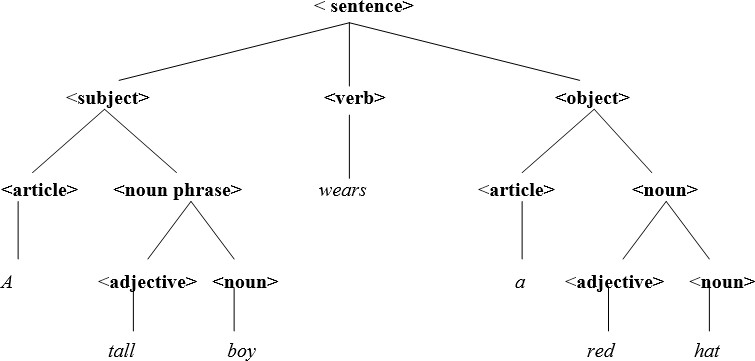
\includegraphics[width=0.8\textwidth]{Gambar/pohonparsing}
	\caption{Pohon \textit{parsing} dari kalimat \textit{A tall boy wears a red hat}}
	\label{fig:g4}
\end{figure}

\section{Validasi Kelompok}

Dalam proses \textit{Clustering}, validasi sistem sudah menjadi sebuah bagian cukup krusial dalam proses membangun model \textit{Clustering}, ukuran dan metode untuk mengevaluasi. Model dibangun menggunakan set data latih dengan sejumlah parameter yang diminta oleh metode yang digunakan. Dalam analisis kelompok, evaluasi dilakukan dengan melakukan pemrosesan data secara alami dengan algoritme yang berjalan sendiri sehingga didapatkan kelompok-kelompok yang terbentuk secara alami pula.

Nilai validasi sangat bermanfaat guna membandingkan apakah algoritme yang digunakan pada penelitian ini menghasilkan tingkat akurasi yang lebih baik dari penelitian-peneliatan sebelumnya yang menggunakan metode selain \textit{Self Organizing Maps} (SOM) yang digunakan untuk \textit{Clustering} suatu data. Pada penelitian ini nilai validasi digunakan apakah dengan menggunakan metode SOM saja sudah cukup menghasilkan tingkat akurasi yang baik atau tidak. Proses validasi dilakukan dengan cara melatih data dan membandingkan kesesuaian hasil \textit{Clustering} data. Validasi kelompok yang digunakan dalam penelitian ini menggunakan \textit{Davies-Bouldin Index} \citep{Dan2015}.

Indeks \textit{silhouette} dan \textit{Davies-Bouldin} adalah dua metode yang digunakan dalam pembelajaran mesin untuk mengevaluasi kualitas kelompok. Indeks \textit{silhouette} digunakan untuk mengevaluasi seberapa baik setiap titik data tergabung dalam kelompok yang sesuai. Ini dilakukan dengan menghitung jarak antara setiap titik data dan kelompok lain yang berdekatan, lalu membandingkannya dengan jarak antara titik data tersebut dan kelompok tempat ia tergabung. Nilai \textit{silhouette} yang lebih tinggi menunjukkan bahwa titik data tersebut lebih baik tergabung dalam \textit{cluster} tempat ia berada. \textit{Davies-Bouldin Index}, di sisi lain, mengevaluasi seberapa baik \textit{cluster-cluster} dipisahkan satu sama lain. Ini dilakukan dengan menghitung rata-rata jarak antara setiap \textit{cluster} dan \textit{cluster} lain yang berdekatan. Nilai yang lebih rendah menunjukkan bahwa \textit{cluster-cluster} lebih baik dipisahkan satu sama lain. Kedua metode ini bertujuan untuk mengevaluasi kualitas \textit{clustering} dan membantu dalam membuat keputusan tentang apakah \textit{clustering} yang dilakukan menghasilkan hasil yang baik atau tidak \citep{Dan2015}.

\section{\textit{Davies-Bouldin Index}}

Validasi kelompok \textit{Davies-Bouldin Index} (DBI) diperkenalkan oleh David L. Davies dan Donald W. Bouldin pada tahun 1979 yang digunakan untuk mengevaluasi kelompok. Validasi internal yang dilakukannya adalah seberapa baik \textit{Clustering} sudah dilakukan dengan menghitung kuantitas dan fitur turunan dari set data.
\textit{Sum of square within cluster} (SSW) dalam sebuah kelompok diformulasikan sebagai berikut: 

\[
SSW_i = \frac{1}{m} \sum_{j=1}^{m_i} d(x_j, c_i)
\]

dengan $mi$ adalah jumlah data yang berada dalam  kelompok ke-$i$, sedangkan $ci$
adalah centroid kelompok ke-$i$.

\textit{Sum of square between cluster} (SSB) dengan mengukur jarak dua kelompok, misalnya kelompok-$i$ dan kelompok-$j$, dengan formula mengukur jarak antara centroid
$ci$ dan $cj$ pada persamaan berikut:

\[
SSB = d(c_i, c_j)
\]

Didefinisikan $R_{ij}$ adalah ukuran rasio seberapa baik nilai perbandingan antara kelompok ke-$i$ dan kelompok ke-$j$. Nilainya didapatkan dari komponen SSW dan SSB. Kelompok yang baik adalah kelompok yang memiliki SSW sekecil mungkin dan SSB yang sebesar mungkin. $R_{ij}$ diformulasikan dengan persamaan berikut:

\[
R_{ij} = \frac{{SSW}_i + {SSW}_j}{{SSB}_{ij}}
\]

Sifat-sifat yang dimiliki $R_{ij}$ sebagai berikut:

\begin{enumerate}
	\item $R_{i,j} \ge 0$
	\item $R_{i,j} = R_{j,i}$
	\item Jika $SSW_j \ge SSW_r$ dan $SSB_{i,j} = SSB_{i,r}$ maka $R_{i,j} > R_{i,r}$
	\item Jika $SSW_j = SSW_r$ dan $SSB_{i,j} \le SSB_{i,r}$ maka $R_{i,j} > R_{i,r}$
\end{enumerate}

Nilai \textit{Davies-Bouldin Index} (DBI) didapatkan dari persamaan berikut: 

\[
DBI = \frac{1}{K} \sum_{i=1}^{K} \max_{j \ne i} (R_{i,j})
\]

$K =$ jumlah kelompok yang digunakan.

Secara esensial, DBI menginginkan nilai sekecil mungkin yang bisa dihasilkan (non-negatif $\geq 0$) untuk menilai baiknya kelompok yang didapat. Nilai yang didapat bisa digunakan sebagai pendukung keputusan untuk menilai jumlah kelompok yang paling cocok digunakan \citep{Dan2015}.

\section{\textit{Silhoutte Coeffisient}}

Pengujian yang dilakukan menggunakan \textit{Silhoutte Coeffisient}. Metode ini berfungsi untuk menguji kualitas dari kelompok yang terbentuk dari hasil metode SOM-MST.
Menurut Romdhoni \citep{Kmeans2018} terdapat 3 langkah yang dilakukan untuk menghitung \textit{Silhoutte Coeffisient} yaitu:

\begin{enumerate}
	\item Hitung rata-rata jarak dari objek $i$ terhadap seluruh objek yang berada dalam satu kelompok.
	\item Hitung rata-rata jarak dari objek $i$ terhadap seluruh objek yang berada pada kelompok lainnya.
	\item Nilai \textit{Silhouette Coefficient} dari objek $i$ menggunakan Persamaan \ref{eq:1}:
	
	\begin{equation}\label{eq:1}
		S_i = \frac{b_i - a_i}{\max(b_i, a_i)}
	\end{equation}
	Dimana:
	\begin{itemize}
		\item $S_i$ = \textit{Silhouette Coefficient} dari objek $i$
		\item $a_i$ = Rata-rata jarak objek $i$ terhadap seluruh objek di dalam kelompok
		\item $b_i$ = Rata-rata jarak objek $i$ terhadap seluruh objek di luar kelompok
	\end{itemize}
	Ukuran nilai \textit{Silhouette Coefficient} \citep{Gentle1991}:
	\begin{enumerate}
		\item $0.7 < SC \le 1$ menyatakan struktur kuat
		\item $0.5 < SC \le 0.7$ menyatakan struktur sedang
		\item $0.25 < SC \le 0.5$ menyatakan struktur lemah
		\item $SC \le 0.25$ menyatakan tidak ada struktur
	\end{enumerate}
\end{enumerate}

